\documentclass[12pt,a4paper]{report}

\usepackage{mathtools}
\usepackage{graphicx}
\usepackage{braket}
\usepackage{amsthm}
\usepackage{lmodern}
\usepackage[utf8]{inputenc}
\usepackage[frenchb]{babel}
\usepackage[T1]{fontenc}
\usepackage{subcaption}
\usepackage{caption}
\usepackage{gensymb}
\usepackage{tikz}
\usepackage{qcircuit}
% \usepackage{a4wide}

\makeatletter
\newcommand\frontmatter{
    \cleardoublepage
    \pagenumbering{roman}
}
\newcommand\mainmatter{
    \cleardoublepage
    \pagenumbering{arabic}
}
\newcommand\backmatter{
  \if@openright
    \cleardoublepage
  \else
    \clearpage
  \fi
}
\makeatother
\newcommand{\norm}[1]{\left\lVert#1\right\rVert}
\newcommand{\Mod}[1]{\ (\mathrm{mod}\ #1)}
\graphicspath{{images/}}

\newtheorem{definition}{Définition}
\newtheorem{pb}{Problème}
\newtheorem{rem}{Remarque}
\newtheorem{ex}{Exemple}

\begin{document}
\begin{titlepage}
    \begin{center}
    
    
\includegraphics[width=0.6\textwidth]{Polytech_Angers.png}\\[1cm]
    
    {\large Master Systèmes Dynamiques et Signaux}\\[0.5cm]
    
    {\large Rapport Bibliographique}\\[0.5cm]
    
    \rule{\linewidth}{0.5mm} \\[0.4cm]
    { \huge \bfseries Informatique Quantique \\[0.4cm] }
    \rule{\linewidth}{0.5mm} \\[1.5cm]
    
    \noindent
    \begin{minipage}{0.4\textwidth}
      \begin{flushleft} \large
        \emph{Auteurs :}\\
        M. Pierre \textsc{Engelstein}\\
         \end{flushleft}
         \end{minipage}%
         \begin{minipage}{0.4\textwidth}
         \begin{flushright} \large
        \emph{Encadrants :}\\
        Dr. Nicolas \textsc{Delanoue}\\
        Pr. François \textsc{Chapeau-Blondeau}\\
         \end{flushright}
    \end{minipage}
    
    \vfill
    
    \large
    \emph{Jury :}
    \begin{tabular}{lc}
        Pr.~Laurent \textsc{Hardouin}\\
        Dr.~Nicolas \textsc{Delanoue}\\
        Pr.~François \textsc{Chapeau-Blondeau}\\
        Pr.~Sébastien \textsc{Lahaye}\\
        Dr.~Mehdi  \textsc{Lhommeau}\\
        Dr.~Remy  \textsc{Guyonneau}\\
    \end{tabular}
    
    \vspace{1cm}
    {\large Version  du \today}
    
    \end{center}
\end{titlepage}

\frontmatter

\section*{Remerciements}

\pagebreak
\tableofcontents

\pagebreak
\listoffigures

\mainmatter

\chapter{Introduction}

Lorem ipsum dolor sit amet, consectetur adipiscing elit, sed do eiusmod tempor incididunt ut labore et dolore magna aliqua. Leo vel orci porta non. Tincidunt ornare massa eget egestas purus viverra accumsan in nisl. Tristique senectus et netus et malesuada fames ac turpis egestas. Varius quam quisque id diam vel quam. Rhoncus urna neque viverra justo nec ultrices. Est velit egestas dui id ornare. Arcu non odio euismod lacinia. Ante metus dictum at tempor. Vulputate sapien nec sagittis aliquam malesuada bibendum arcu vitae elementum. Non nisi est sit amet facilisis magna etiam. Quis commodo odio aenean sed adipiscing diam. Etiam erat velit scelerisque in. Tortor id aliquet lectus proin nibh nisl condimentum id. At auctor urna nunc id cursus metus aliquam.

Nec sagittis aliquam malesuada bibendum arcu vitae. Amet nisl purus in mollis. Ac tincidunt vitae semper quis lectus. Ac felis donec et odio pellentesque diam volutpat commodo sed. Ipsum dolor sit amet consectetur adipiscing elit pellentesque. Tortor vitae purus faucibus ornare suspendisse sed nisi. Tristique risus nec feugiat in fermentum posuere urna nec tincidunt. Egestas purus viverra accumsan in nisl nisi scelerisque eu. Ac odio tempor orci dapibus ultrices. Molestie ac feugiat sed lectus vestibulum mattis ullamcorper velit. Interdum velit laoreet id donec ultrices. Donec adipiscing tristique risus nec feugiat in fermentum posuere urna. Porttitor leo a diam sollicitudin. Cras sed felis eget velit aliquet sagittis. Ut etiam sit amet nisl purus in. Viverra suspendisse potenti nullam ac tortor vitae purus faucibus ornare. Lorem ipsum dolor sit amet consectetur adipiscing elit ut aliquam.

\chapter{Informatique quantique: éléments de base}

\section{Postulats de base}

On pose 3 postulats, servant de base aux raisonnements qui suivront. Ces postulats sont des hypothèses de travail, mais confirmés jusqu'a présent par les expériences.

\subsection{Etat d'un système quantique}
Un système quantique peut être représenté par un vecteur d'état, de la même manière qu'un système physique classique. On le représente par la notation de Dirac, notée de la forme $\ket{\psi}$. Ce vecteur d'état est necessairement de norme 1 (la somme des modules au carré vaut 1). On peut distinguer deux types d'états pour un système quantique: les états de base, ou \textbf{états purs}, formant une base vectorielle, et les états superposés. Ces états superposés correspondent à une combinaison linéaire des états purs. On peut écrire généralement un état quantique de la façon suivante:

\begin{equation}
    \ket{\psi} = \displaystyle\sum_{i} c_i \ket{k_i},
\end{equation}

avec les $\ket{k_i}$ états purs, et les $c_i$ respectant $ \displaystyle\sum_{i} |c_i|^2 = 1$ pour la normalité du vecteur d'état.

\medbreak

Dans le cadre de l'informatique quantique, on utilise le système quantique le plus simple, appelé \textbf{qubit}. Ce système quantique est composé de deux états purs, $\ket{0}$ et $\ket{1}$, et des états superposés. Similairement à l'informatique classique, où on travaille sur le système physique le plus élémentaire - le bit - en quantique on travaille sur le système physique quantique élémentaire - le qubit. On dispose des mêmes états purs, mais l'informatique quantique apporte les états \textit{intermédiaires} superposés. Dans la base canonique $\{\ket{0}, \ket{1}\}$, on note un qubit de la façon suivante: $\ket{\psi} = \alpha \cdot \ket{0} + \beta \cdot \ket{1}$.

\subsection{Mesure projective}
Que se passe-t-il quand on mesure un système quantique ? On a évoqué au dessus la notion de superposition des états. L'expérience montre que, lorsqu'on va mesurer un système quantique, on va mesurer au hasard un des états de base, avec comme probabilité le carré du coefficient correspondant.

Mathématiquement, la mesure effectue une projection de l'état du système sur un des états de base dont il est composé. Par exemple, si on a un qubit dans l'état $\ket{\psi} = \frac{1}{\sqrt{2}}\ket{0} + \frac{1}{\sqrt{2}}\ket{1}$, alors la probabilité de mesurer 0, c'est à dire de projeter le système dans l'état pur $\ket{0}$ est $|\frac{1}{\sqrt{2}}|^2 = \frac{1}{2}$; et de même pour l'état pur $\ket{1}$. On a donc exactement la même probabilité de mesurer 0 que de mesurer 1.

Il faut noter que, lorsqu'on fait la mesure, on projete réellement le système quantique dans l'état pur. Concrètement, si on a un état superposé qu'on mesure, il se place dans l'état pur qu'on mesure, et toutes les mesures successives qu'on fera sur ce qubit donneront le même résultat. La mesure fait donc perdre l'état qu'on avait auparavant.

\subsection{Dynamique du système}
Comme n'importe quel système physique, on peut faire évoluer un système quantique dans le temps. Ici apparaissent deux propriétés. Tout d'abord, il découle du premier postulat que la dynamique d'un système quantique est necessairement unitaire. En effet, un système quantique doit, pour être valide, avoir une norme de 1, et donc l'évolution d'un système quantique d'un premier état vers un autre doit conserver cette unitarité. Cela veut dire que la matrice représentant l'évolution du système quantique doit respecter la propriété suivante:

\begin{equation}
    U^{\dagger}U = UU^{\dagger} = I,
\end{equation}

avec $U$ la matrice d'évolution du système, $U^{\dagger}$ la matrice conjuguée transposée de $U$, et $I$ l'identité.

Une deuxième propriété est également posée, ne découlant pas des deux postulats précédents. La dynamique d'un système quantique doit être aussi linéaire. Ainsi, on pourrait penser que n'importe quelle évolution unitaire serait valable, mais l'expérience nous montre que non, il faut en plus qu'elle soit linéaire.

\section{Vers une informatique quantique}
A partir de ces 3 postulats de base, on peut commencer à comprendre comment se construit l'informatique quantique, et quels sont les apports sur l'informatique classique.

\subsection{Multiples qubits}
On a vu la définition d'un qubit. Cela nous permet d'étendre ce système quantique élémentaire à des systèmes composés de multiples qubits. En informatique classique, on travaille quasi systématiquement sur des mots binaires plutôt que des bits uniques; l'équivalent est vrai en quantique. Pour cela, les systèmes quantiques, et donc les qubits, sont munis d'une opération: le produit tensoriel. Quand on veut effectuer une combinaison de deux qubits, cela revient à faire un produit tensoriel des états des deux qubits individuels. Par exemple, si nous disposons de deux qubits ayant pour valeur $\ket{\psi_1} = \ket{0}$ et $\ket{\psi_2} = \ket{1}$, alors on peut écrire le 2-qubit combinaison des deux de la façon suivante:


\begin{equation}
    \ket{\psi} = \ket{0} \tens{} \ket{1},
\end{equation}

qu'on écrit généralement sous la forme plus simple:

\begin{equation}
    \ket{\psi} = \ket{01}.
\end{equation}

Prenons un 2-qubit formé par la combinaison de 2 qubits:

\begin{align*}
\ket{\psi} &= (\alpha_1\cdot\ket{0} + \beta_1\cdot\ket{1}) \otimes (\alpha_2\cdot\ket{0} + \beta_2\cdot\ket{1}) \\
&= \alpha_1\alpha_2 \ket{0} \otimes \ket{0} + \alpha_1\beta_2 \ket{0} \otimes \ket{1} + \beta_1\alpha_2 \ket{1} \otimes \ket{0} + \beta_1\beta_2 \ket{1} \otimes \ket{1} \\
&= \gamma_1 \ket{00} + \gamma_2 \ket{01} + \gamma_3 \ket{10} + \gamma_4 \ket{11}
\end{align*}

On peut donc, si on a un 2-qubit combinaison linéaire de tout les états de bases, le séparer en deux qubits individuels, sur lesquels on va pouvoir agir.

\medbreak

Considérons maintenant le 2-qubit suivant:

\[
\ket{\psi} = \gamma_1 \ket{00} + \gamma_2 \ket{11}
\]

Il parait évident alors qu'on ne peut pas séparer ce 2-qubit en produit tensoriel de 2 qubits individuels. Dans ce cas, on dit que les deux qubits sont \textbf{intriqués} et donc non séparables.


\subsection{Portes quantiques}
Dans la représentation d'état classique, et spécifiquement en informatique, on peut faire évoluer l'état au travers de portes. En informatique classique, on dispose ainsi de portes élémentaires telles que \texttt{AND}, \texttt{NOT}, \texttt{OR}, etc. 

De la même manière, en respectant le troisième postulat posé précédement, on peut construire des portes logiques quantiques, les combiner, afin de créer des circuits quantiques. En informatique quantique, on distingue donc plusieurs portes élémentaires, utilisés dans beaucoup de circuit:

\begin{enumerate}
    \item La porte de Hadamard $H$. Elle permet de passer un qubit d'un état pur $\ket{0}$ à l'état superposé $\frac{1}{\sqrt{2}}\ket{0} + \frac{1}{\sqrt{2}}\ket{1}$, ou de l'état pur $\ket{1}$ à l'état superposé $\frac{1}{\sqrt{2}}\ket{0} - \frac{1}{\sqrt{2}}\ket{1}$. Elle est très utilisée en début de circuit pour préparer les qubits entrants dans un état permettant l'évaluation parallèle de toutes les entrées;
    \item Les portes de Pauli $X$, $Y$ et $Z$ permettant d'effectuer des rotations aux états des qubits;
    \item La porte de Toffoli, équivalent d'un \texttt{NON} booléen, est une porte universelle quantique. Elle permet donc de construire l'ensemble des autres portes faisables.
\end{enumerate}

Un exemple de circuit est le suivant: On dispose d'un 3-qubit dans l'état $\ket{000}$. Au départ, on applique à ces trois qubits une porte de Hadamard, qui les fait se retrouver dans des états équilibrés. On arrive donc à un 3-qubit qui est équilibré entre chacun de ses états purs. On applique ensuite deux portes de Pauli $Z$, un au premier qubit, et un au troisième. Cela est effectivement faisable puisqu'a la sortie des portes de hadamard, les 3 qubits ne sont pas intriqués. On applique de la même façon 3 portes de Hadamard à la sortie, puis on mesure. 

\centerline{
  \Qcircuit @C=1em @R=.7em {
    & \lstick{\ket{0}} & \gate{H} \barrier[-1.25em]{2} & \gate{Z} \barrier[-1.25em]{2} & \gate{H} & \meter & \qwa \\
    & \lstick{\ket{0}} & \gate{H} & \qw & \gate{H} & \meter & \qwa \\
    & \lstick{\ket{0}} & \gate{H} & \gate{Z} & \gate{H} & \meter & \qwa
  }
}

L'avantage du quantique bien montré ici: Les deux portes du milieu vont faire changer l'état des qubits, mais en parallèle: on fait évoluer le système simultanément pour tout les états purs qui nous intéressent, puisqu'ils sont superposés.


% \subsection{Formalisme mathématique}

% \subsubsection*{Qubit unique}

% Le qubit possède deux états de base, correspondant aux états des bits classiques. On les représente par $\ket{0}$, correspondant à l'état $0$ classique, et par $\ket{1}$ pour l'état $1$ classique. A la différence d'un bit classique, un qubit peut également prendre une infinité d'autres états que ses états de base. La question se pose alors de la mesure: que va-t-on mesurer quand un qubit est dans un état autre que $\ket{0}$ ou $\ket{1}$ ? C'est là qu'apparaissent les bizarreries de la mécanique quantique. La mesure va donner au hasard $0$ ou $1$, suivant des probabilités définies.

% Pour représenter ce comportement, on note un qubit de la façon suivante:

% \begin{equation}
% \ket{\psi} = \alpha \cdot \ket{0} + \beta \cdot \ket{1}
% \end{equation}

% Le qubit est alors représenté par une combinaison linéaire des deux états de base $\ket{0}$ et $\ket{1}$, suivant les coefficients complexes $\alpha$ et $\beta$. Ces coefficients représentent les amplitudes de probabilité suivant lesquelles on va mesurer $\ket{0}$ ou $\ket{1}$.

% Ces deux coefficients complexes doivent absolument respecter la propriété suivante:

% \begin{equation}
% \norm{\alpha}^2 + \norm{\beta}^2 = 1
% \end{equation}    

% \subsubsection*{Multiples qubits}

% Une fois ces éléments posés, on peut commencer à travailler avec plusieurs qubits, notés n-qubits. Mathématiquement, une combinaison de qubits correspond à un produit tensoriel de deux vecteurs.

% Prenons les qubits $\ket{0}$ et $\ket{1}$. La combinaisons en un 2-qbits est donc:

% \begin{equation}
%     \ket{\psi} = \ket{0} \tens{} \ket{1}
% \end{equation} 

% qu'on peut écrire plus simplement:

% \begin{equation}
%     \ket{\psi} = \ket{01}
% \end{equation}

% Un 2-qubit a donc 4 états de bases, représentés par: $\{\ket{00},\ket{01}, \ket{10}, \ket{11} \}$, et peut donc être la combinaison linéaire de n'importe quel de ces états de base

% \subsubsection*{Intrication}
% Prenons un 2-qubit formé par la combinaison de 2 qubits:

% \begin{align*}
% \ket{\psi} &= (\alpha_1\cdot\ket{0} + \beta_1\cdot\ket{1}) \otimes (\alpha_2\cdot\ket{0} + \beta_2\cdot\ket{1}) \\
% &= \alpha_1\alpha_2 \ket{0} \otimes \ket{0} + \alpha_1\beta_2 \ket{0} \otimes \ket{1} + \beta_1\alpha_2 \ket{1} \otimes \ket{0} + \beta_1\beta_2 \ket{1} \otimes \ket{1} \\
% &= \gamma_1 \ket{00} + \gamma_2 \ket{01} + \gamma_3 \ket{10} + \gamma_4 \ket{11}
% \end{align*}

% On peut donc, si on a un 2-qubit combinaison linéaire de tout les états de bases, le séparer en deux qubits individuels, sur lesquels on va pouvoir agir.

% \medbreak

% Considérons maintenant le 2-qubit suivant:

% \[
% \ket{\psi} = \gamma_1 \ket{00} + \gamma_2 \ket{11}
% \]

% Il parait évident alors qu'on ne peut pas séparer ce 2-qubit en produit tensoriel de 2 qubits individuels. Dans ce cas, on dit que les deux qubits sont \textbf{intriqués} et donc non séparables.

% \section{Représentation géométrique}

% \section{Programmer un processeur quantique}
\chapter{Algorithme de Deutsch-Jozsa}

\section{Problème à résoudre}
Soit une fonction $f$ booléenne définie par 
\[
  \begin{array}{llll}
    f :  &  \{0, 1\}^n              & \to       & \{ 0, 1 \} \\
         &  (x_0, x_1, \dots , x_n) & \mapsto   &  y = f(x_0, x_1, \dots , x_n), 
  \end{array}  
\]

\begin{definition}
  Une fonction booléenne $f$ est dite équilibrée si $f$ retourne 0
  pour la moitié de ses entrées.
\end{definition}

\begin{definition}
  Une fonction est dite constante si elle retourne une constante pour
  toutes ses entrées.
\end{definition}


\begin{rem}
  Avec $n$ un entier et comme les fonctions booléennes sont à valeur
  dans $\{0,1\}$, il n'existe que deux fonctions constantes $f_0$ et
  $f_1$.
\end{rem}

\begin{ex}
  Soit $f$ la fonction booléenne $f : \{0,1\}^2 \to \{0,1\}$ définie
  par la table de vérité suivante :
\[
  \begin{array}{|c|c|}
    \hline
   (x_1, x_2) & f(x_1,x_2) \\
    \hline
    (0,0) & 0 \\
    \hline
    (0,1) & 1 \\
    \hline
    (1,0) & 1 \\
    \hline
    (1,1) & 0 \\
    \hline
  \end{array}
\]
Cette fonction est équilibrée. On notera qu'elle correspond au
classique ``ou exclusif''. Cette fonction pourrait être représentée
par le vecteur de ces valeurs : $(0,1,1,0)$. Elle peut aussi être
codée en listant les emplacements où elle est vraie, ici $\{1,2\}$.
\end{ex}

% \begin{rem}
%   Dénombrer les fonctions équilibrées revient à dénombrer les façons
%   de placer le symbole le symbole $1$ dans la moitié des cases d'un
%   vecteur de taille $2^n$. Avec les emplacements, cela revient à
%   dénombrer l'ensemble de sous-ensembles de $\{0, \dots, 2^{n}-1 \}$
%   qui ont pour cardinal $2^n / 2$. Finalement, il a donc
%   ${\displaystyle {2^n \choose 2^{n-1}}}$ fonctions équilibrées. Ce qui fait
%   \[ {\displaystyle {2^n \choose 2^{n-1}}} = \frac{(2^n)!}{(2^{n-1})!(2^n-2^{n-1})!} = \frac{(2^n)!}{((2^{n-1})!)^2}.  \]

%   On notera que la proportion des fonctions équilibrées sur l'ensemble
%   des $2^{2^n}$ fonctions booléennes de $n$ variables diminue très
%   rapidement avec $n$.
% \end{rem}


\begin{pb}[Deutsch-Jozsa]
Etant donnée une fonction $f$ qui est soit équilibrée, soit constante.
Le problème de Deutsch-Jozsa est de déterminer si $f$ est constante ou
équilibrée.  
\end{pb}

\subsection{Solution classique}
Dans le cas classique, il faut effectuer au pire $2^{n-1}+1$
évaluations pour déterminer si $f$ est constante ou équilibrée. Tout
d'abord, dès que deux évaluations sont différentes, $f$ est
nécessairement équilibrée. De plus, si après avoir évalué $2^{n-1}$
entrées et obtenu la même valeur, une évaluation supplémentaire nous
permet de connaitre dans quelle catégorie $f$ se trouve.

\subsection{Solution quantique}
Dans le cas quantique, ce problème se résout en une seule évaluation
quantique de $f$.

\begin{figure}[htbp]
    \centering
    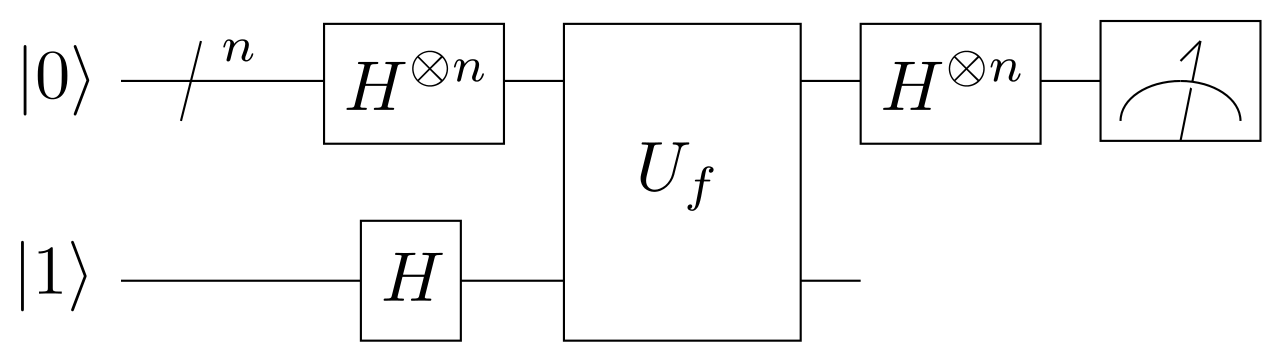
\includegraphics[scale=0.2]{DJ/Deutsch-Jozsa_Algorithm.png}
    \caption{Schéma de l'algorithme}
    \label{fig:univerise}
\end{figure}

\subsubsection{Initialisation}
On commence avec :
$\ket{u_0} = (\ket{0}^{\bigotimes n}) \otimes \ket{1}$
: n-qubits à $\ket{0}$ et 1-qubit à $\ket{1}$

\subsubsection{Etape 1}

On applique une porte de Hadamard à $\ket{u_0}$ pour avoir un état équiprobable:
$\ket{u_1} = H\ket{u_0} = \frac{1}{\sqrt{2^{n + 1}}}
\displaystyle\sum_{x=0}^{2^n-1} \ket{x}(\ket{0} - \ket{1})$

\subsubsection{Etape 2}
On applique l'oracle quantique suivant à $\ket{u_1}$:
\[ o : \ket{x}\ket{y}\mapsto \ket{x}\ket{y\oplus f(x)}. \]

Posons $x$, on est alors dans l'une des deux situations disjointes suivantes :
\begin{itemize}
\item $f(x) = 0$,
\item $f(x) = 1$.
\end{itemize}

Analysons chacune de ces situations, tout d'abord si $f(x) = 0$ alors
%Prenons le cas à 1 qubit:
\[
o : \ket{x}(\ket{0} - \ket{1}) \mapsto \ket{x}(\ket{0} - \ket{1})
\]
Autrement dit $\ket{x}(\ket{0} - \ket{1}$ est un  point fixe de $o$.

Dans l'autre situation, on a $f(x) = 1$ et on en déduit
\[
o : \ket{x}(\ket{0} - \ket{1}) \mapsto \ket{x}(\ket{1} - \ket{0})
\]
Autrement dit, dans ce cas, le vecteur $\ket{x}(\ket{0} - \ket{1})$
est envoyé sur son opposé via $o$.

Finalement, les deux cas précédents peuvent être résumé sous la forme suivante
\[
o : \ket{x}(\ket{0} - \ket{1}) \mapsto (-1)^{f(x)}\ket{x}(\ket{0} - \ket{1})
\]

Par linéarité, on en déduit :

\begin{equation}\ket{u_2} = \frac{1}{\sqrt{2^{n + 1}}} 
\displaystyle\sum_{x=0}^{2^n-1} (-1)^{f(x)}\ket{x}(\ket{0} - \ket{1}) 
\end{equation}

On peut ignorer le dernier qubit ($\ket{0} - \ket{1}$) comme il est
constant. Finalement, on en déduit :
\begin{equation}
\ket{u_2} = \frac{1}{\sqrt{2^{n + 1}}}
\displaystyle\sum_{x=0}^{2^n-1} (-1)^{f(x)}\ket{x}
\end{equation}

\subsubsection{Etape 3}

Maintenant qu'on a appliqué notre oracle, on est toujours dans un état
"probabiliste", et en mesurant nous n'obtiendrons pas une réponse
exacte à notre problème. L'objectif est donc maintenant de ramener les
solutions sur un état déterminé pour obtenir la réponse
systématique. En appliquant la porte de Hadamard, on va pouvoir forcer
un état à apparaître pour un type de fonction $f$, et le forcer à
disparaître dans l'autre cas, ce qui nous permet d'avoir une réponse
systématique sur le type de la fonction : est-elle équilibrée ou bien constante ?

On réapplique une porte Hadamard à chaque qubit sortant, ce qui donne:

\[ \ket{u_3} = \frac{1}{\sqrt{2^{n}}}
\displaystyle\sum_{x=0}^{2^n-1} (-1)^{f(x)} \left( \frac{1}{\sqrt{2^{n}}} \displaystyle\sum_{y=0}^{2^n-1} (-1)^{x.y}\ket{y} \right) \]

Par linéarité, on a :
\begin{equation}
  \label{eq:1}
  \ket{u_3} = \frac{1}{2^{n}}
  \displaystyle\sum_{x=0}^{2^n-1} \displaystyle\sum_{y=0}^{2^n-1}(-1)^{f(x)} (-1)^{x.y}\ket{y}  
\end{equation}

La probabilité $|p|$ de mesurer $\ket{0}^{\bigotimes n}$ est donc : 
\begin{equation}
  \label{eq:2}
  |\frac{1}{2^{n}}\displaystyle\sum_{x=0}^{2^n-1}(-1)^{f(x)}|
\end{equation}

avec $p = \frac{1}{2^{n}}\displaystyle\sum_{x=0}^{2^n-1}(-1)^{f(x)}$.

Si on a une fonction $f(x)$ constante, alors chaque élément de la
somme retourne la même valeur (1 ou -1 suivant que $f(x)$ retourne 0
ou 1), la somme va donc valoir $\pm 2^{n}$. Dans le cas où la fonction
est équilibrée, on va avoir autant de 1 que de -1, la somme est donc
nulle.

On a donc les valeurs suivantes dépendant du type de $f(x)$ :
\begin{enumerate}
  \item Si $f(x)$ est constante :  $p = \pm \frac{1}{2^n} \times 2^{n} = \pm 1$,
  \item Si $f(x)$ est équilibrée : $p = \pm \frac{1}{2^n} \times 0 = 0$.
\end{enumerate}

Dans le cas constant, on ne peut donc que mesurer $\ket{0}^{\bigotimes n}$ puisqu'il a une probabilité de 1 d'apparaître. Dans le cas équilibré, on ne mesure jamais $\ket{0}^{\bigotimes n}$ puisque sa probabilité est nulle.

On en conclut que, lorsqu'on effectue une mesure, si on tombe sur $\ket{0}^{\bigotimes n}$ alors la fonction est constante, sinon elle est équilibrée.

%'objectif de cette dernière étape est de passer 

\subsection{Exemple}

Prenons une fonction $f$ comme définie précédemment avec $n=2$, sans
savoir si elle est constante ou équilibrée.

\subsubsection{Etape 1}


On commence avec $\ket{u_0} = \ket{001}$. La première étape est
l'application de la porte d'hadamard à $\ket{u_0}$:

\begin{align}
\ket{u_1} &= H\ket{u_0} = H\ket{0} \otimes H\ket{0} \otimes H\ket{1} \nonumber \\
& = \frac{1}{2\sqrt{2}} \left( (\ket{0} + \ket{1})\otimes(\ket{0} + \ket{1})\otimes(\ket{0} - \ket{1}) \right) \nonumber \\
 & = \frac{1}{2\sqrt{2}}\{\ket{000} - \ket{001} + \ket{010} - \ket{011} + \ket{100} - \ket{101} + \ket{110} - \ket{111}\} \nonumber \\
& = \frac{1}{2\sqrt{2}}\{\ket{00}(\ket{0} - \ket{1}) + \ket{01}(\ket{0} - \ket{1}) + \ket{10}(\ket{0} - \ket{1}) + \ket{11}(\ket{0} - \ket{1})\}
\end{align}

%On peut factoriser le tout par $(\ket{0} - \ket{1})$: 
%$

\subsubsection{Etape 2: oracle quantique}

On applique à $\ket{u_1}$ l'oracle quantique $\ket{x}\ket{y}\rightarrow\ket{x}\ket{y\oplus f(x)}:$

\begin{align*}
\ket{u_2}  =  \frac{1}{2\sqrt{2}}  & \ket{00}(\ket{0 \oplus f(00)} - \ket{1 \oplus f(00)}) + \\
& \ket{01}(\ket{0 \oplus f(01)} - \ket{1 \oplus f(01)}) + \\
& \ket{10}(\ket{0 \oplus f(10)} - \ket{1 \oplus f(10)}) + \\
& \ket{11}(\ket{0 \oplus f(11)} - \ket{1 \oplus f(11)})  \\
\end{align*}


On peut alors réécrire l'équation de la façon suivante: 



\begin{align*}
  \ket{u_2} = \frac{1}{2\sqrt{2}} & (-1)^{f(00)} \ket{00}  (\ket{0} - \ket{1}) + \\
&(-1)^{f(01)} \ket{01}  (\ket{0} - \ket{1}) + \\
&(-1)^{f(10)} \ket{10}  (\ket{0} - \ket{1}) + \\
&(-1)^{f(11)} \ket{11}  (\ket{0} - \ket{1}) 
\end{align*}

Par la suite, on va appliquer une porte de Hadamard à $\ket{u_2}$. Le qubit $\ket{0} - \ket{1}$ donne $\ket{1}$ par la cette porte, il est donc constant par rapport à $\ket{u_0}$. On peut donc le retirer de l'équation, ce qui nous donne pour $\ket{u_2}$ :

\begin{equation}
  \label{eq:3}
\ket{u_2} = \frac{1}{2\sqrt{2}} \left( (-1)^{f(00)} \ket{00} + (-1)^{f(01)} \ket{01} + (-1)^{f(10)} \ket{10} + (-1)^{f(11)} \ket{11} \right) 
\end{equation}


Matriciellement, on peut donc écrire

\begin{equation}
  \label{eq:4}
\ket{u_2} = \left(  \begin{array}{cccc}
     (-1)^{f(00)}  &0 & 0 &0 \\
     0 & (-1)^{f(01)} & 0 &0 \\
     0 &0 & (-1)^{f(10)} &0 \\
     0 &0 & 0 & (-1)^{f(11)} \\
        \end{array}
      \right)
      \left(  \begin{array}{c}
                1 \\
                1 \\
                1 \\
                1 
              \end{array}
      \right)      
\end{equation}


\subsubsection{Etape 3: porte de Hadamard}

On applique donc une porte de hadamard à $\ket{u_2}$:
\begin{equation}
  \label{eq:5}
\ket{u_3} = \frac{1}{2\sqrt{2}} H \left( (-1)^{f(00)} \ket{00} + (-1)^{f(01)} \ket{01} + (-1)^{f(10)} \ket{10} + (-1)^{f(11)} \ket{11} \right) 
\end{equation}

Nous sommes sur une porte de hadamard pour 2 qubits, ce qui donne
la relation matricielle suivante pour $\ket{u_3}$:

\begin{align}
\ket{u_3} &=
\frac{1}{4\sqrt{2}} 
\begin{bmatrix}
  1 & 1 & 1 & 1 \\
  1 & -1 & 1 & -1 \\
  1 & 1 & -1 & -1 \\
  1 & -1 & -1 & 1 \\
\end{bmatrix}
\begin{bmatrix}
  (-1)^{f(00)} \\ (-1)^{f(01)} \\ (-1)^{f(10)} \\ (-1)^{f(11)}
\end{bmatrix} , \nonumber \\ 
 &= \frac{1}{4\sqrt{2}} 
\begin{bmatrix}
  (-1)^{f(00)} + (-1)^{f(01)} + (-1)^{f(10)} + (-1)^{f(11)} \\
  (-1)^{f(00)} - (-1)^{f(01)} + (-1)^{f(10)} - (-1)^{f(11)} \\
  (-1)^{f(00)} + (-1)^{f(01)} - (-1)^{f(10)} - (-1)^{f(11)} \\
  (-1)^{f(00)} - (-1)^{f(01)} - (-1)^{f(10)} + (-1)^{f(11)} \\
\end{bmatrix}.
\end{align}

Si f est constante , alors
$(-1)^{f(00)} = (-1)^{f(01)} = (-1)^{f(10)} = (-1)^{f(11)}$. En
fonction du fait que $f=0$ ou bien $f=1$:

\begin{equation}
  \label{eq:6}
\ket{u_3}=
\frac{1}{\sqrt{2}} 
\begin{bmatrix}
  1 \\ 0 \\ 0 \\ 0
\end{bmatrix}  \text{ ou bien }
\ket{u_3}=
\frac{1}{\sqrt{2}} 
\begin{bmatrix}
  -1 \\ 0 \\ 0 \\ 0
\end{bmatrix}.
\end{equation}
On a donc une probabilité de $1$ de mesurer l'état $\ket{00}$.

En revanche, si f est équilibrée, la moitié des valeurs vont
valoir $(-1)^{0} = 1$ et l'autre moitié $(-1)^{1} = -1$. La première
ligne du vecteur $\ket{u_3}$ donne donc systématiquement 0, on ne mesure donc
jamais l'état $\ket{00}$.

\section{Visualisation géométrique}
Reprenons cet algorithme avec $n=4$ qubits et affichons l'évolution des états des qubits avec des sphères de bloch.

\subsection{Fonction constante $f_0(x)$ = 0}
\medbreak
\begin{figure}[ht]
  \begin{subfigure}[b]{0.6\textwidth}
      \centering
      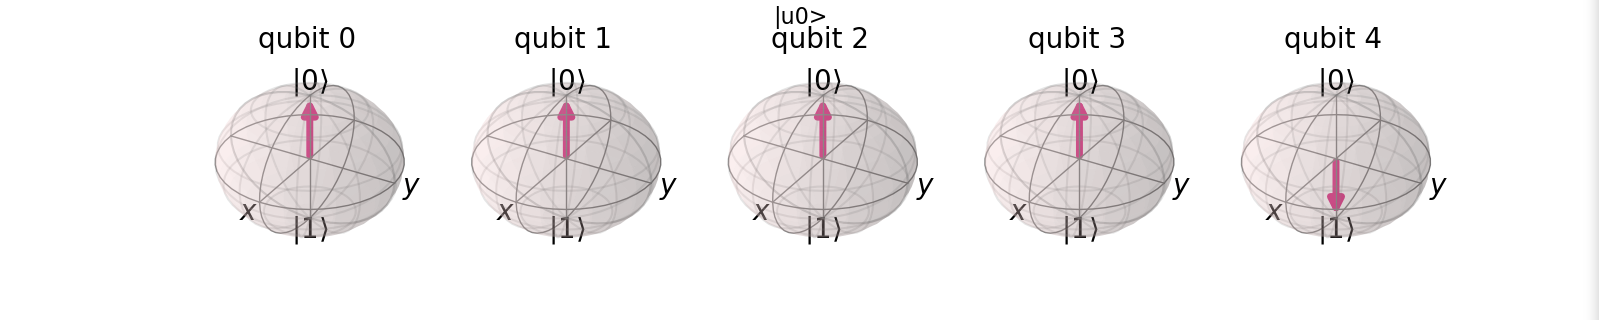
\includegraphics[width=\textwidth]{DJ/visualization_constant_1_u0.png}
      \caption{$\ket{u0}=\ket{0001}$}
  \end{subfigure}
  \begin{subfigure}[b]{0.6\textwidth}
      \centering
      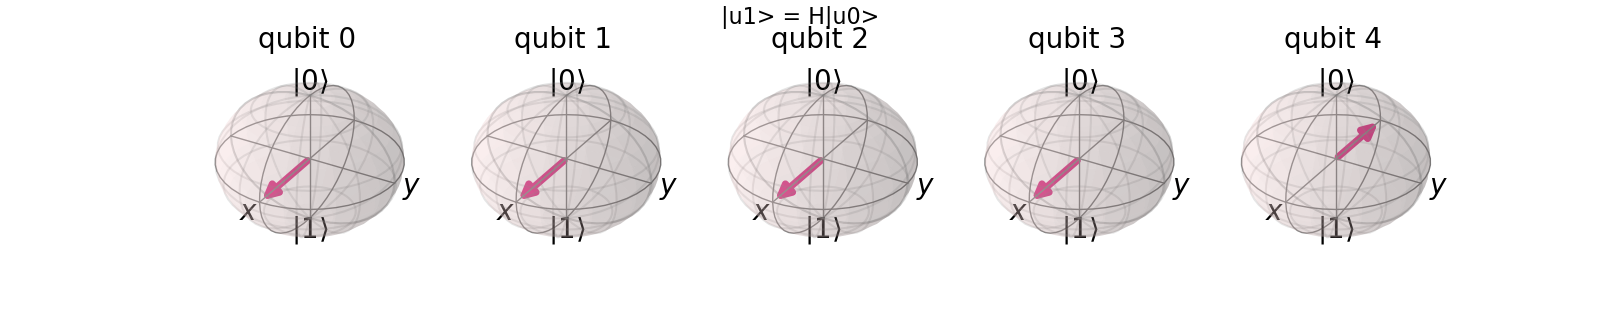
\includegraphics[width=\textwidth]{DJ/visualization_constant_1_u1.png}
      \caption{$\ket{u1}=H\ket{u0} = \ket{+++-}$}
  \end{subfigure}
  \begin{subfigure}[b]{0.6\textwidth}
      \centering
      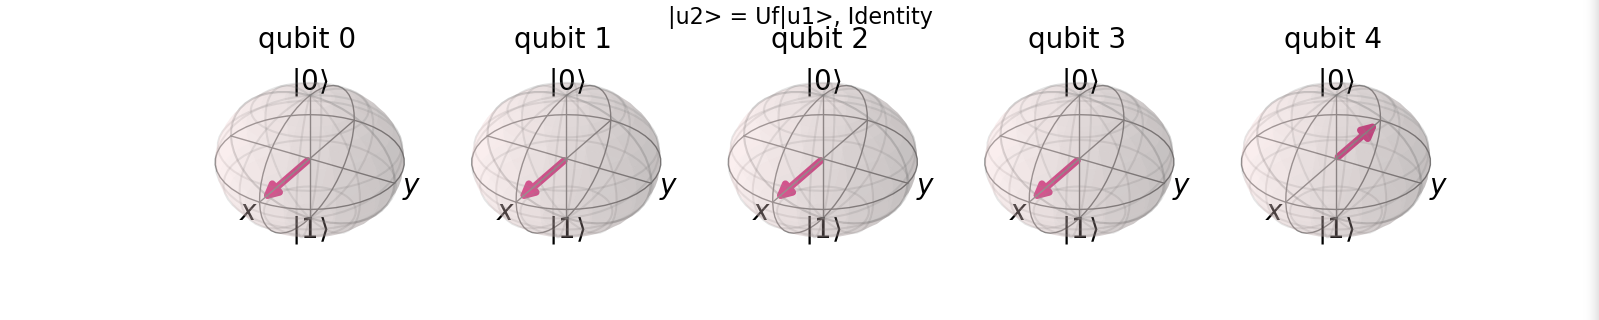
\includegraphics[width=\textwidth]{DJ/visualization_constant_1_u2.png}
      \caption{$\ket{u2}=U_f\ket{u1}$}
  \end{subfigure}
  \begin{subfigure}[b]{0.6\textwidth}
    \centering
    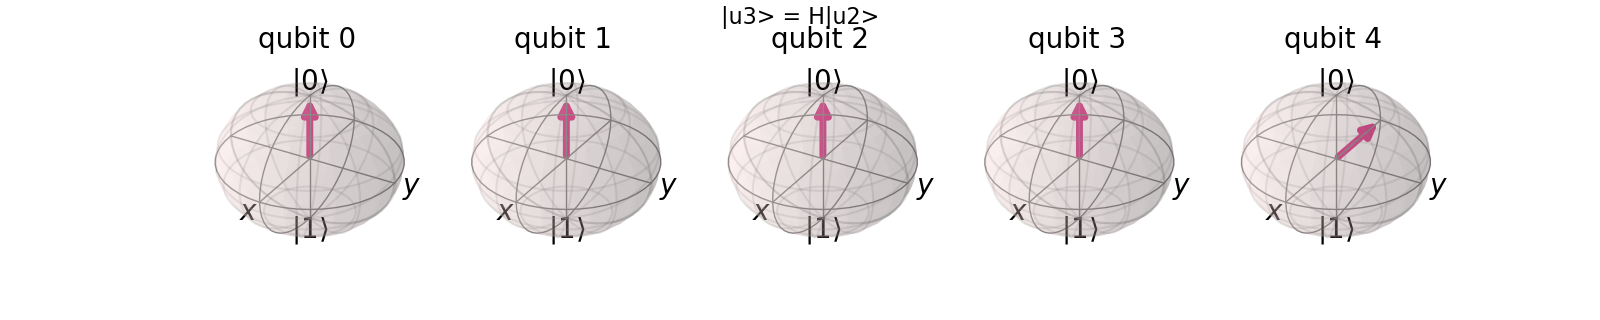
\includegraphics[width=\textwidth]{DJ/visualization_constant_1_u3.png}
    \caption{$\ket{u3}=H\ket{u2}$}
\end{subfigure}
     \caption{Evolution des états pour une fonction f constante, vecteurs d'états séparés}
\end{figure}

\pagebreak

On peut aussi visualiser ces figures avec une shère de bloch représentant les 5 qubits ensembles avec les phases:

\begin{figure}[bth]
  \begin{subfigure}[b]{0.25\textwidth}
      \centering
      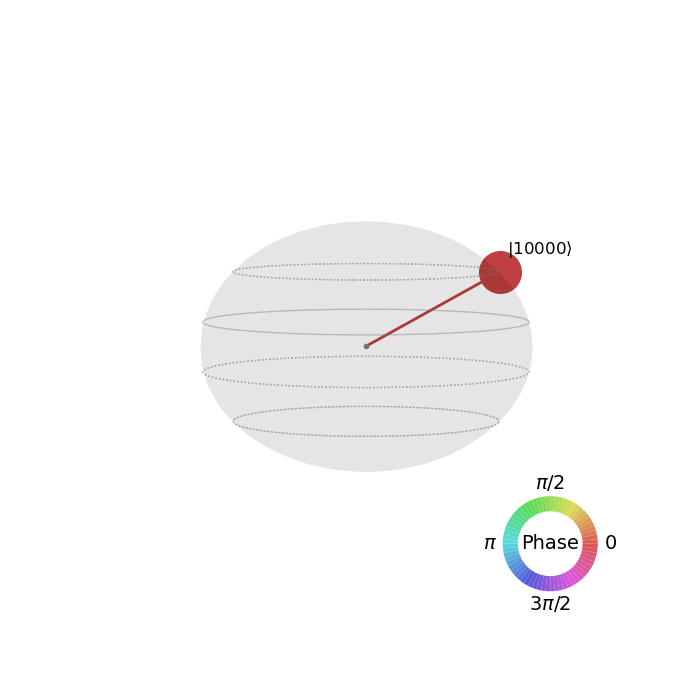
\includegraphics[width=\textwidth]{DJ/visualization_constant_2_u0.png}
      \caption{$\ket{u0}=\ket{0001}$}
  \end{subfigure}
  \begin{subfigure}[b]{0.25\textwidth}
      \centering
      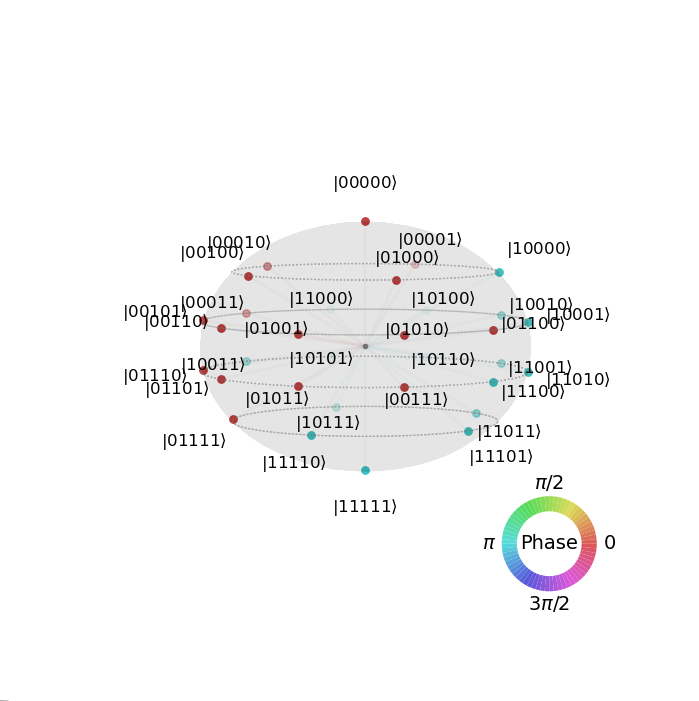
\includegraphics[width=\textwidth]{DJ/visualization_constant_2_u1.png}
      \caption{$\ket{u1}=H\ket{u0}$}
  \end{subfigure}
  \begin{subfigure}[b]{0.25\textwidth}
      \centering
      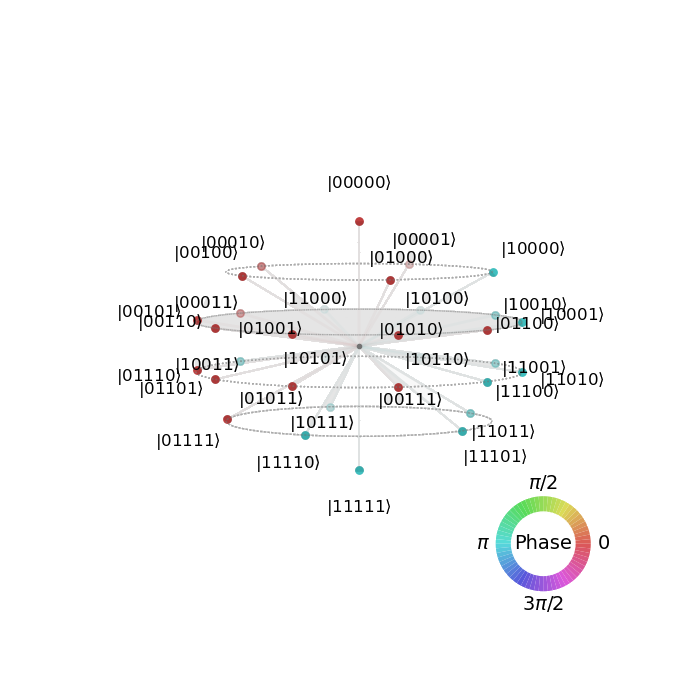
\includegraphics[width=\textwidth]{DJ/visualization_constant_2_u2.png}
      \caption{$\ket{u2}=U_f\ket{u1}$}
  \end{subfigure}
  \begin{subfigure}[b]{0.25\textwidth}
    \centering
    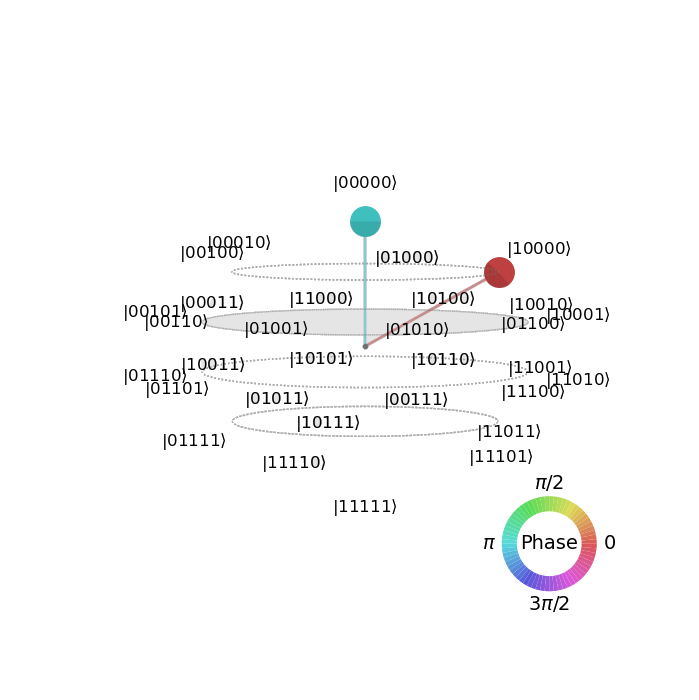
\includegraphics[width=\textwidth]{DJ/visualization_constant_2_u3.png}
    \caption{$\ket{u3}=H\ket{u2}$}
\end{subfigure}
     \caption{Evolution des états pour une fonction f constante}
\end{figure}

On voit ici l'ensemble des états que prends le registre de sortie. Dans le cas constant, on se retrouve bien à mesure exclusivement la valeur 0 (pour rappel, on ne mesure pas le dernier qubit qui est constant à 1). Pour les deux étapes intermédiaires, on visualise bien qu'on se retrouve dans une certaine superposition des états possibles.

\pagebreak

\subsection{Fonction équilibrée quelconque $f_1(x)$}
Les deux figues suivantes présentent la même visualisation, pour une fonction équilibrée:

\begin{figure}[ht]
  \begin{subfigure}[b]{0.6\textwidth}
      \centering
      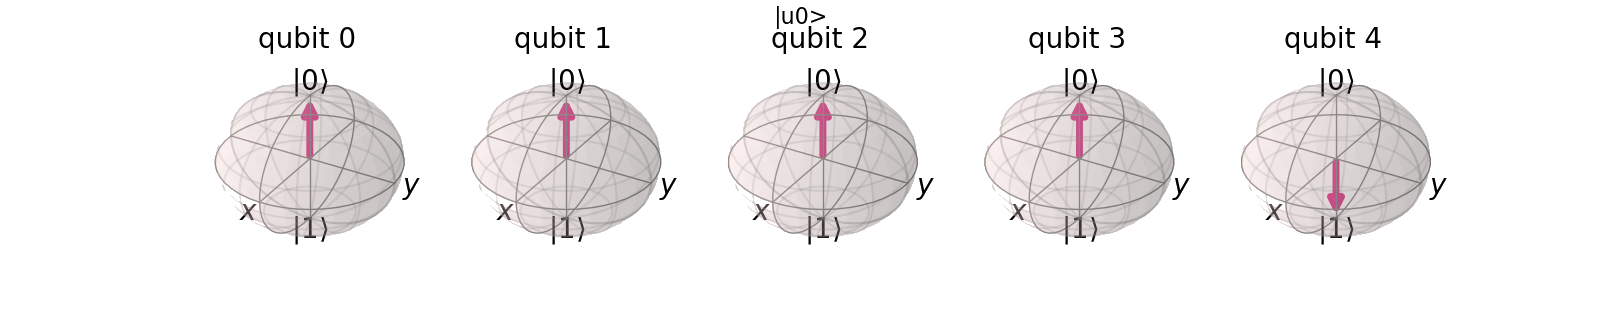
\includegraphics[width=\textwidth]{DJ/visualization_eq_1_u0.png}
      \caption{$\ket{u0}=\ket{0001}$}
  \end{subfigure}
  \begin{subfigure}[b]{0.6\textwidth}
      \centering
      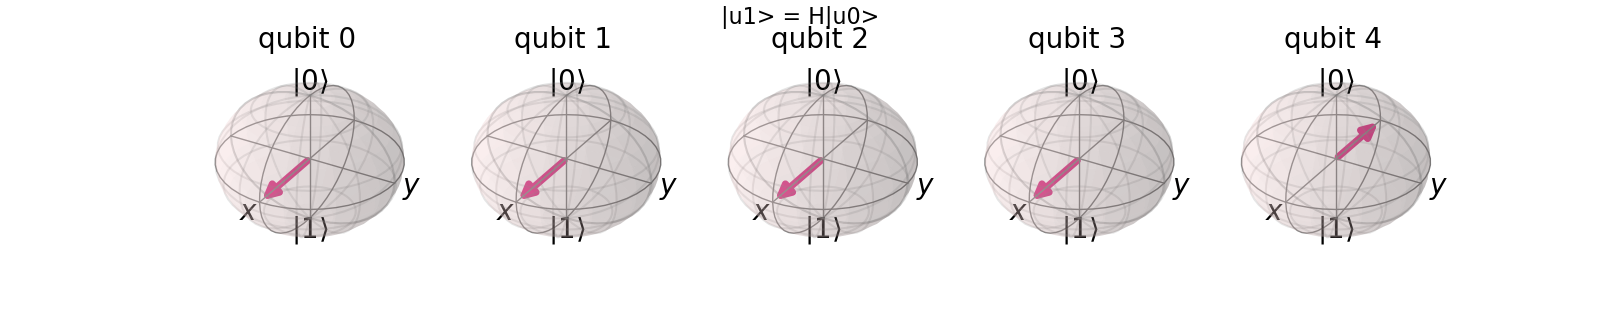
\includegraphics[width=\textwidth]{DJ/visualization_eq_1_u1.png}
      \caption{$\ket{u1}=H\ket{u0}$}
  \end{subfigure}
  \begin{subfigure}[b]{0.6\textwidth}
      \centering
      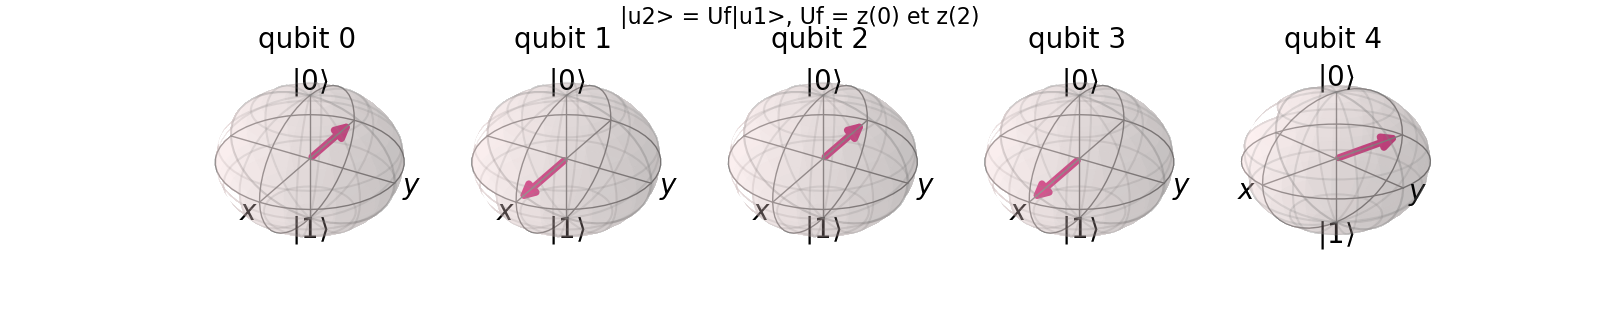
\includegraphics[width=\textwidth]{DJ/visualization_eq_1_u2.png}
      \caption{$\ket{u2}=U_f\ket{u1}$}
  \end{subfigure}
  \begin{subfigure}[b]{0.6\textwidth}
    \centering
    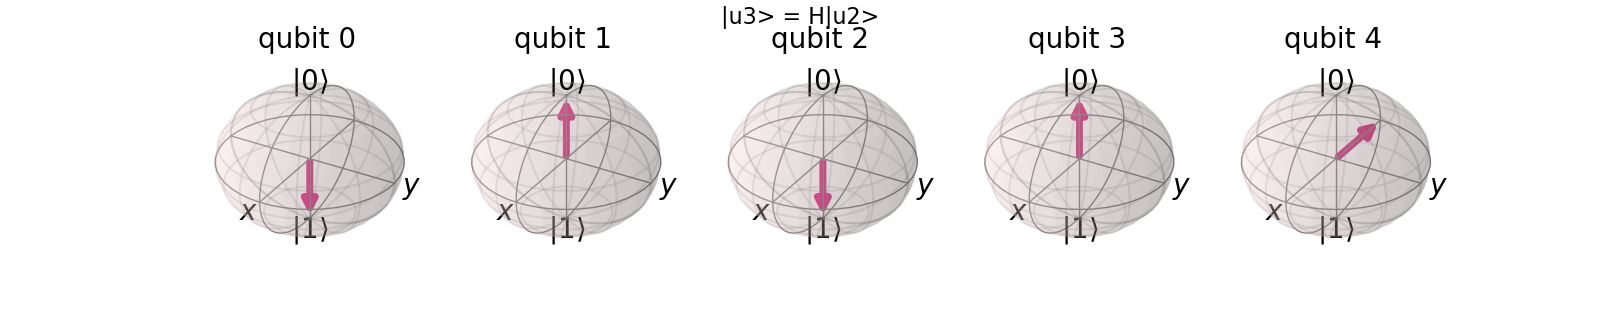
\includegraphics[width=\textwidth]{DJ/visualization_eq_1_u3.png}
    \caption{$\ket{u3}=H\ket{u2}$}
\end{subfigure}
     \caption{Evolution des états pour une fonction f équilibrée, vecteurs d'états séparés}
\end{figure}

\begin{figure}[bth]
  \begin{subfigure}[b]{0.23\textwidth}
      \centering
      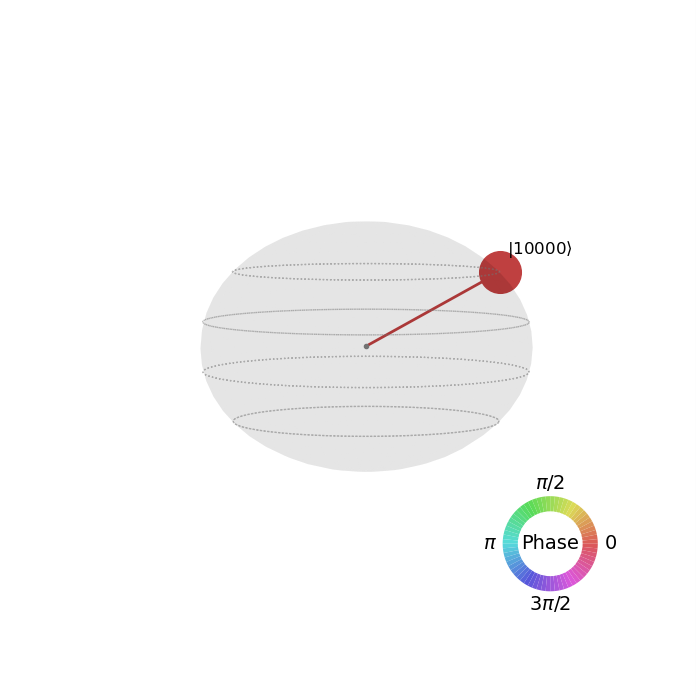
\includegraphics[width=\textwidth]{DJ/visualization_eq_2_u1.png}
      \caption{$\ket{u0}=\ket{0001}$}
  \end{subfigure}
  \begin{subfigure}[b]{0.23\textwidth}
      \centering
      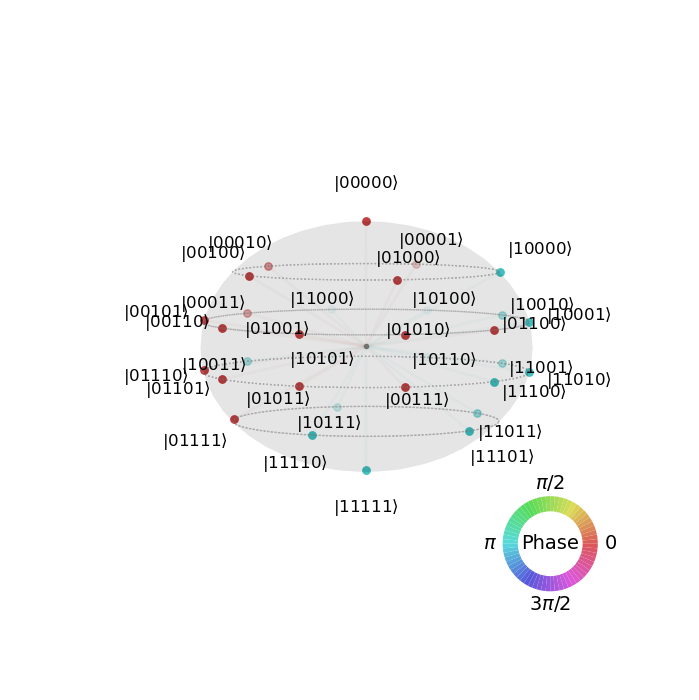
\includegraphics[width=\textwidth]{DJ/visualization_eq_2_u2.png}
      \caption{$\ket{u1}=H\ket{u0}$}
  \end{subfigure}
  \begin{subfigure}[b]{0.23\textwidth}
      \centering
      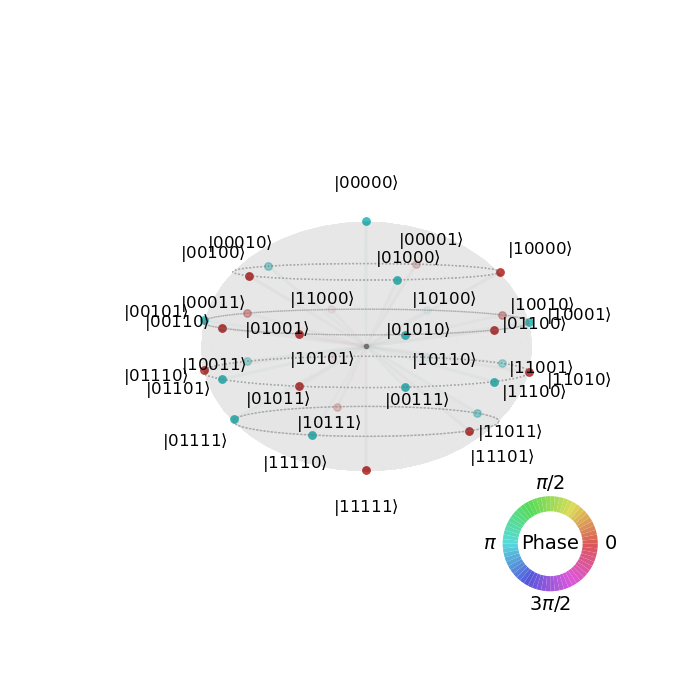
\includegraphics[width=\textwidth]{DJ/visualization_eq_2_u3.png}
      \caption{$\ket{u2}=U_f\ket{u1}$}
  \end{subfigure}
  \begin{subfigure}[b]{0.23\textwidth}
    \centering
    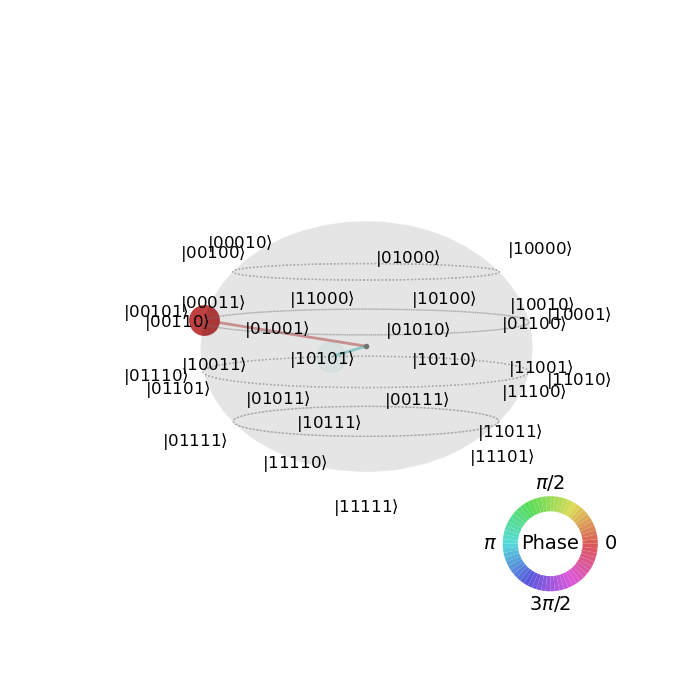
\includegraphics[width=\textwidth]{DJ/visualization_eq_2_u4.png}
    \caption{$\ket{u3}=H\ket{u2}$}
\end{subfigure}
     \caption{Evolution des états pour une fonction f équilibrée}
\end{figure}

On voit bien sur cette figure que dans le cas d'une fonction équilibrée, l'état va se situer à un des points indiqués sur la sphère de Bloch mais jamais sur le point 0. 

\chapter{Algorithme dérivé de Deutsch-Jozsa: Bernstein-Vazirani}
\section{Problème à résoudre}

Soient $x$ et $s$ tels que $x, s \in \{0, 1\}^n$.

On pose une fonction $f$ définie par:
\[
  \begin{array}{llll}
    f :  &  x              & \to     & y = s \cdot x \Mod{2} = x_1 s_1 + x_2 s_2 + \dots + x_n s_n \\
    f:   &  \{0, 1\}^n     & \to     & \{0, 1\},
  \end{array}  
\]

\begin{ex}
  Soit $s$ le mot booléen suivant: $s = 10$. La fonction $f$ a donc la table de véritée suivante:
\[
  \begin{array}{|c|c|c|}
    \hline
   (x_1, x_2) & s & f(x_1,x_2) \\
    \hline
    (0,0) & 10 & 0 \\
    \hline
    (0,1) & 10 & 0 \\
    \hline
    (1,0) & 10 & 1 \\
    \hline
    (1,1) & 10 & 1 \\
    \hline
  \end{array}
\]
On observe que le résultat est de 1 pour les entrées $(x_1, x_2)$ où l'emplacement des $1$ correspond à ceux de $s$.
\end{ex}

\begin{pb}[Bernstein-Vazirani]
Etant donné un mot $s$ secret, et la fonction $f$ implémentant l'opération décrite précédemment, comment peut on retrouver $s$ en le moins d'évaluations de $f$ possibles ?
\end{pb}

\subsection{Solution classique}
Dans le cas classique, on va devoir évaluer au pire toutes les valeurs possibles de $s$ pour trouver sa valeur, soit $n$ évaluations de $f$. C'est un algorithme de complexité $\mathcal{O}(n)$

\subsection{Solution quantique}
Dans le cas quantique, ce problème se résout en une seule évaluation
quantique de $f$. L'algorithme reprends celui de Deutsch-Jozsa en changeant la fonction appliquée dans l'oracle quantique.

\subsubsection{Initialisation}
On commence avec :
$\ket{u_0} = (\ket{0}^{\bigotimes n})$
: n-qubits à $\ket{0}$

\subsubsection{Etape 1}

On applique une porte de Hadamard à $\ket{u_0}$ pour avoir un état équiprobable:
$\ket{u_1} = H\ket{u_0} = \frac{1}{\sqrt{2^n}}
\displaystyle\sum_{x=0}^{2^n-1} \ket{x}$

\subsubsection{Etape 2}
On applique l'oracle quantique suivant à $\ket{u_1}$:
\[ o : \ket{x}\ket{y}\mapsto \ket{x}\ket{y\oplus (s \cdot x \Mod{2})}. \]

En suivant exactement le même raisonnement que pour Deutsch-Jozsa, on arrive à l'expression suivante: 

\begin{equation}\ket{u_2} = \frac{1}{\sqrt{2^n}}
\displaystyle\sum_{x=0}^{2^n-1} (-1)^{s \cdot x \Mod{2}}\ket{x} 
\end{equation}

\subsubsection{Etape 3}

De la même façon à Deutsch-Jozsa, on applique une porte Hadamard à chaque qubit sortant, ce qui donne:

\[ \ket{u_3} = \frac{1}{\sqrt{2^{n}}}
\displaystyle\sum_{x=0}^{2^n-1} (-1)^{s \cdot x \Mod{2}} \left( \frac{1}{\sqrt{2^{n}}} \displaystyle\sum_{y=0}^{2^n-1} (-1)^{x.y}\ket{y} \right) \]

\begin{align}
  \ket{u_3} &= \frac{1}{\sqrt{2^{n}}}\displaystyle\sum_{x=0}^{2^n-1} (-1)^{s \cdot x \Mod{2}} \left( \frac{1}{\sqrt{2^{n}}} \displaystyle\sum_{y=0}^{2^n-1} (-1)^{x.y}\ket{y} \right) \\
  & = \frac{1}{2^{n}} \displaystyle\sum_{x=0}^{2^n-1} \displaystyle\sum_{y=0}^{2^n-1} (-1)^{(s \cdot x \Mod{2}) + x.y} \ket{y}
  \end{align}

Et on peut prouver que $\frac{1}{2^{n}} \displaystyle\sum_{x=0}^{2^n-1} \displaystyle\sum_{y=0}^{2^n-1} (-1)^{(s \cdot x \Mod{2}) + x.y} \ket{y}$ est égal à $\ket{s}$.
% (\textit{à faire ...})

\subsection{Exemple}

Prenons par exemple $s=(10)_2 = 2_{10}$, soit $f(x) = 2 \cdot x \Mod{2}$
\subsubsection*{Etape 1: porte de Hadamard}

On commence avec $\ket{u_0} = \ket{00}$. La première étape est
l'application de la porte d'hadamard à $\ket{u_0}$:

\begin{align}
\ket{u_1} &= H\ket{u_0} = H\ket{0} \otimes H\ket{0} \\
& = \frac{1}{2} \left( (\ket{0} + \ket{1})\otimes(\ket{0} + \ket{1}) \right) \\
 & = \frac{1}{2}\{\ket{00} + \ket{01} + \ket{10} + \ket{11}\}
\end{align}

%On peut factoriser le tout par $(\ket{0} - \ket{1})$: 
%$

\subsubsection*{Etape 2: oracle quantique}

On applique à $\ket{u_1}$ l'oracle quantique $\ket{x}\ket{y}\rightarrow\ket{x}\ket{y\oplus (s \cdot x \Mod{2})} = :$

\begin{align*}
  \ket{u_2} &= \frac{1}{2}((-1)^{10 \cdot 00 \Mod{2}} \ket{00} + (-1)^{10 \cdot 01 \Mod{2}} \ket{01} + (-1)^{10 \cdot 10 \Mod{2}} \ket{10} + (-1)^{10 \cdot 11 \Mod{2}} \ket{11}) \\
  &= \frac{1}{2}((-1)^{0} \ket{00} + (-1)^{0} \ket{01} + (-1)^{1} \ket{10} + (-1)^{1} \ket{11}) \\
  &= \frac{1}{2} (\ket{00} + \ket{01} - \ket{10} - \ket{11})
\end{align*}

\subsubsection*{Etape 3: porte de Hadamard}

On applique donc une porte de hadamard à $\ket{u_2}$:
\begin{equation}
  \label{eq:5}
\ket{u_3} = \frac{1}{2} H \left( (\ket{00} + \ket{01} - \ket{10} + \ket{11}) \right) 
\end{equation}

Nous sommes sur une porte de hadamard pour 2 qubits, ce qui donne
la relation matricielle suivante pour $\ket{u_3}$:

\begin{align}
\ket{u_3} &=
\frac{1}{4} 
\begin{bmatrix}
  1 & 1 & 1 & 1 \\
  1 & -1 & 1 & -1 \\
  1 & 1 & -1 & -1 \\
  1 & -1 & -1 & 1 \\
\end{bmatrix}
\begin{bmatrix}
  1 \\ 1 \\ -1 \\ -1
\end{bmatrix} , \\ 
 &= \frac{1}{4} 
\begin{bmatrix}
  0 \\
  0 \\
  4 \\
  0 \\
\end{bmatrix}.
\end{align}

Lors de la mesure, on va obtenir l'état $\ket{10}$ avec une probabilité de 1, qui était bien notre mot binaire $s$ de départ.

On peut observer que, lors de l'application de la porte de Hadamard à $\ket{u_2}$, on obtient la superposition d'état suivante: $\ket{00} + \ket{01} - \ket{10} - \ket{11}$. Cela correspond à la troisième ligne de la matrice de Hadamard, correspondant au $\ket{s}$ voulu. Dans tout les cas, peut importe le $s$ choisi, on obtiendra une superposition d'état correspondant à une des lignes de la matrice, forçant à 0 les probabilités de tout les états sauf de celui indiqué.

\subsection{Implémentation du circuit}

\subsubsection*{Circuit global}
L'implémentation du circuit quantique pour cet algorithme est très similaire à celui de Deutsch-Jozsa, à la différence qu'on a un qubit de moins:

\centerline{
  \Qcircuit @C=1em @R=.7em {
    & \gate{H} & \multigate{2}{U_f} & \gate{H} & \meter & \qw \\
    & \gate{H} & \ghost{U_f}& \gate{H} & \meter & \qw \\
    & \gate{H} & \ghost{U_f} & \gate{H} & \meter & \qw
  }
}
\subsubsection*{Implémentation de l'oracle}

Prenons le cas où $n=2$. La matrice correspondant à la porte $U_f$ va avoir 4 possibilité pour obtenir, comme on l'a dit lors de l'exemple, une des 4 lignes de la matrice de Hadamard:
\[
U_{f_{00}} = 
\begin{bmatrix}
  1 & 0 & 0 & 0 \\
  0 & 1 & 0 & 0 \\
  0 & 0 & 1 & 0 \\
  0 & 0 & 0 & 1 \\
\end{bmatrix}
, U_{f_{01}} = 
\begin{bmatrix}
  1 & 0 & 0 & 0 \\
  0 & -1 & 0 & 0 \\
  0 & 0 & 1 & 0 \\
  0 & 0 & 0 & -1 \\
\end{bmatrix}
,U_{f_{10}} = 
\begin{bmatrix}
  1 & 0 & 0 & 0 \\
  0 & 1 & 0 & 0 \\
  0 & 0 & -1 & 0 \\
  0 & 0 & 0 & -1 \\
\end{bmatrix}
, U_{f_{11}} = 
\begin{bmatrix}
  1 & 0 & 0 & 0 \\
  0 & -1 & 0 & 0 \\
  0 & 0 & -1 & 0 \\
  0 & 0 & 0 & 1 \\
\end{bmatrix}
\]

On remarque que ces quatres matrices sont en fait des produits tensoriels de deux matrices correspondant à des portes à 1 qubit:

\[
  I = 
  \begin{bmatrix}
    1 & 0 \\
    0 & 1 \\
  \end{bmatrix}
  , Z = 
  \begin{bmatrix}
    1 & 0 \\
    0 & -1 \\
  \end{bmatrix}
\]

Pour $n=2$, on a $s \in \{00, 01, 10, 11\}$. En reprenant les matrices correspondantes, on obtient les produits tensoriels suivant:

\[
U_{f_{00}} = I \otimes I
, U_{f_{01}} = I \otimes Z
,U_{f_{10}} = Z \otimes I
, U_{f_{11}} = Z \otimes Z
\]

On peut généraliser sur l'implémentation en disant:

\begin{align}
  U_f = \displaystyle \bigotimes_{i=0}^{n} U_i, \; U_i = \begin{cases}
    I  & \text{si } s_i = 0 \\
    Z  & \text{si } s_i = 1 \\
  \end{cases}
\end{align}

Un exemple d'implémentation complète serait alors (pour $s = 101$):

\centerline{
  \Qcircuit @C=1em @R=.7em {
    & \lstick{\ket{0}} & \gate{H} \barrier[-1.25em]{2} & \gate{Z} \barrier[-1.25em]{2} & \gate{H} & \meter & \qw \\
    & \lstick{\ket{0}} & \gate{H} & \qw & \gate{H} & \meter & \qw \\
    & \lstick{\ket{0}} & \gate{H} & \gate{Z} & \gate{H} & \meter & \qw
  }
}
\chapter{Algorithme de Grover}

\section{Rappels d'algèbre: projection et reflection}

Soient deux vecteurs $\overrightarrow{u}$ et $\overrightarrow{u}$, avec $\overrightarrow{v}$ normalisé.

\begin{definition}
  La matrice de projection $P$ de $\overrightarrow{u}$ sur $\overrightarrow{v}$ est définie par $P = \overrightarrow{v} \cdot \overrightarrow{v^T}$.
\end{definition}

\begin{definition}
  La matrice de reflection $R$ de $\overrightarrow{u}$ par rapport à $\overrightarrow{v}$ est définie par $R = 2 \overrightarrow{v} \cdot \overrightarrow{v^T} - I$.
\end{definition}

\begin{ex}
Prenons $\overrightarrow{u}=\begin{bmatrix}2\\3\end{bmatrix}$ et $\overrightarrow{v}=\begin{bmatrix}1\\-2\end{bmatrix}$.

On projete $\overrightarrow{u}$ sur $\overrightarrow{v}$:

$P = \frac{\overrightarrow{v} \cdot \overrightarrow{v^T}}{\norm{v}^2} = \begin{bmatrix}\frac{1}{\sqrt{5}} & \frac{-2}{\sqrt{5}}\\\frac{-2}{\sqrt{5}} & \frac{4}{\sqrt{5}}\end{bmatrix}$
\medbreak
Soit: $\overrightarrow{u_v} = P\overrightarrow{u} = \begin{bmatrix}-0.8\\1.6\end{bmatrix}$
\end{ex}

\begin{ex}
Prenons à nouveau $\overrightarrow{u}=\begin{bmatrix}2\\3\end{bmatrix}$ et $\overrightarrow{v}=\begin{bmatrix}1\\-2\end{bmatrix}$.
On effectue une reflection de $\overrightarrow{u}$

$R = 2 \times \frac{\overrightarrow{v} \cdot \overrightarrow{v^T}}{\norm{v}^2} - I = 2 \times \begin{bmatrix}\frac{1}{\sqrt{5}} & \frac{-2}{\sqrt{5}}\\\frac{-2}{\sqrt{5}} & \frac{4}{\sqrt{5}}\end{bmatrix} - \begin{bmatrix}1 & 0 \\ 0 & 1\end{bmatrix}$
\end{ex}

La première étape est la double projection $2\times P$, ce qui donne le vecteur $\begin{bmatrix}-1.6\\3.2\end{bmatrix}$.

La deuxième étape est d'enlever le vecteur initial, ce qui donne le vecteur $\overrightarrow{u_R} = \begin{bmatrix}-3.6\\0.2\end{bmatrix}$.

On peut vérifier les angles $\theta_{UV}$ et $\theta_{VU_R}$:

$\theta_{UV} = \arccos({\frac{u \cdot v}{\norm{u}\norm{v}}}) = \arccos({\frac{-4}{\sqrt{13} \times \sqrt{5}}}) = 119.7\degree$

$\theta_{VU_R} = \arccos({\frac{v \cdot u_R}{\norm{v}\norm{u_R}}}) = \arccos({\frac{-4}{\sqrt{5} \times \sqrt{13}}}) = 119.7\degree$

Les deux angles sont bien égaux, on a effectué une reflection.

\begin{tikzpicture}
  \draw[thin,gray!40] (-4,-3) grid (3,4);
  \draw[<->] (-3,0)--(3,0) node[right]{$x$};
  \draw[<->] (0,-3)--(0,4) node[above]{$y$};
  \draw[line width=1pt,blue,-stealth](0,0)--(2, 3) node[anchor=south west]{$\boldsymbol{\overrightarrow{u}}$};
  \draw[line width=1pt,red,-stealth](0,0)--(1,-2) node[anchor=north east]{$\boldsymbol{\overrightarrow{v}}$};
  \draw[line width=1pt,green,-stealth](0,0)--(-0.8,1.5) node[anchor=north east]{$\boldsymbol{\overrightarrow{u_v}}$};
  \draw[line width=1pt,gray!200,dashed](2, 3) -- (-0.8,1.5){};
  \draw[line width=1pt,gray!200,dashed](-0.8,1.5)--(-1.6,3.0) node[anchor=north east]{$\boldsymbol{2 \times P}$};
  \draw[line width=1pt,gray!200,dashed](-1.6,3.0)--(-3.6,0.2) node[anchor=north east]{};
  \draw[line width=1pt,green,-stealth](0,0)--(-3.6,0.2) node[anchor=north east]{$\boldsymbol{\overrightarrow{u_R} = (2 \times P - I)\overrightarrow{u}}$};
\end{tikzpicture}

\section{Problème à résoudre}
Soit une base de données non triée à $N$ entrées. Nous voulons trouver un algorithme permettant de chercher efficacement un enregistrement dans cette base.


\subsection{Principe de l'algorithme}
L'algorithme de Grover permet de résoudre ce problème en quantique, en disposant de $N$ qubits intriqués pour calculer $2^N$ état 
(donc si on a $N$ entrées dans la base, il nous faut $log_2(N)$ qubits intriqués). Dans le cas de cet algorithme, on considère le problème suivant:
\medbreak
On marque $\{0, 1, 2, ..., N-1\}$ les enregistrements de la base de données, et on dénote $\omega$ l'état inconnu recherché. On dispose de la fonction suivante:

$f(x) = 
 \begin{cases}
   1, & \text{si x vérifie le critère} \; \omega \\
   0, & \text{sinon}
 \end{cases}
$

A la fin, on obtient un set de résultat. Or, lors de la mesure on va avoir au hasard une des solutions suivant les probabilités de chaque état, alors qu'on cherche
juste à savoir la (ou les) bonnes solutions. On rajoute donc une amplification d'amplitude permettant d'augmenter les probabilités des bons résultats et de diminuer
celles des mauvais.


\subsubsection*{Initialisation}

On commence avec :
$\ket{u_0} = (\ket{0}^{\bigotimes n}) \otimes \ket{1}$
: n-qubits à $\ket{0}$ et 1-qubit à $\ket{1}$

\subsubsection*{Etape 1}

On applique une porte de Hadamard à $\ket{u_0}$ pour avoir un état équiprobable:
$\ket{u_1} = H\ket{u_0} = \frac{1}{\sqrt{2^{n + 1}}}
\displaystyle\sum_{x=0}^{2^n-1} \ket{x}(\ket{0} - \ket{1})$

On pose alors $\ket{s} = \frac{1}{\sqrt{2^n}} \displaystyle\sum_{x=0}^{2^n-1} \ket{x}$

\subsubsection*{Etape 2: opérateurs de Grover}

On définit les deux opérateurs suivants:

$U_w = I - 2\ket{w}\bra{w}$, avec $w$ état cible correspondant à la solution du problème (amplitude de 1 sur l'état visé, amplitude nulle sur le reste)

$U_s = 2\ket{s}\bra{s} - I$

\begin{rem}
  On reconnait ici que ces deux opérateurs sont semblables à la reflection vue dans la partie 1.
\end{rem}

\paragraph*{Inversion d'amplitude}

L'opérateur $U_w$ effectue l'inversion de l'amplitude de l'état cible, tandis que l'opérateur $U_s$ effectue le miroir des amplitudes par rapport à la moyenne.

On applique $U_w$ puis $U_s$:

$U_w \ket{s} = (I - 2 \ket{w}\bra{w})\ket{s} \nonumber = \ket{s} - 2 \ket{w}\braket{w|s}$

Or, $\braket{w|s}$ est un produit scalaire. $\ket{w}$ est définit plus haut, et $\ket{s}$ est l'état équiprobable obtenu après la porte de hadamard. Le résultat est donc $\braket{w|s} = \frac{1}{\sqrt{2^n}}$. On peut donc réécrire:

$\ket{u_3} = U_w \ket{s} = \ket{s} - \frac{2}{\sqrt{2^n}}\ket{w}$

\paragraph*{Miroir à la moyenne}
On applique ensuite l'opérateur $U_s$ au résultat de $U_w$. On peut voir qu'en pratique $U_s$ effectue un miroir de $\ket{u_3}$ par rapport à $\ket{s}$.

\begin{align}
  U_s\ket{u_3} 
  &= (2\ket{s}\bra{s} - I)(\ket{s} - \frac{2}{\sqrt{2^n}}\ket{w}) \nonumber \\
  &= 2\ket{s}\braket{s|s} - \ket{s} - \frac{4}{\sqrt{2^n}} \ket{s} \braket{s|w} + \frac{2}{\sqrt{2^n}}\ket{w} \nonumber \\
  &= 2\ket{s} - \ket{s} + \frac{4}{\sqrt{2^n}} \times \frac{1}{\sqrt{2^n}} \ket{s} + \frac{2}{\sqrt{2^n}}\ket{w} \nonumber \\
  &= \ket{s} - \frac{4}{2^n} \ket{s} + \frac{2}{\sqrt{2^n}}\ket{w} \nonumber \\
  \ket{u_4}&=\frac{2^n - 4}{2^n}\ket{s} + \frac{2}{\sqrt{2^n}}\ket{w}
\end{align}

% \chapter{Quantum Fourier Transform}

\end{document}